\documentclass{article}
\usepackage{iclr2027_conference,times}

\usepackage{amsmath,amssymb,mathtools}
\usepackage{booktabs,tabularx,array,multirow}
\usepackage{graphicx}
\usepackage[dvipsnames]{xcolor}
\usepackage{microtype}
\usepackage{tikz}
\usetikzlibrary{arrows.meta,positioning}
\usepackage{hyperref}
\usepackage{url}
\usepackage[nameinlink,noabbrev]{cleveref}

\definecolor{censureblue}{HTML}{1F5A7A}
\definecolor{censureteal}{HTML}{177E75}
\definecolor{censureorange}{HTML}{C96B2C}
\definecolor{lightblue}{HTML}{EAF3F8}
\definecolor{lightorange}{HTML}{FBEFE6}

\newcommand{\method}{\textsc{Censure}}
\newcommand{\E}{\mathbb{E}}
\newcommand{\gap}{\Delta_{\mathrm{mask}}}
\newcommand{\Vbeh}{V_b}
\newcommand{\Vstar}{V_\star}
\newcommand{\Hb}{H_b}
\newcommand{\Hs}{H_\star}
\newcolumntype{Y}{>{\centering\arraybackslash}X}

\hypersetup{
    colorlinks=true,
    linkcolor=censureblue,
    citecolor=censureblue,
    urlcolor=censureteal
}

\title{When Guardrails Hide Risk:\\
First-Divergence Auditing for Tool-Using Language Agents}

\author{Anonymous Authors}

% Keep this commented for anonymous review.
% \iclrfinalcopy

\begin{document}
\maketitle

\begin{abstract}
Action guards can reduce the harm observed during an agent evaluation while leaving the
underlying actor's propensity for unsafe action unresolved. Evaluating only the deployed,
guarded trajectory can therefore conflate actor safety with successful intervention. We study
this problem using a paired full-trajectory audit: for every frozen task and seed, we
independently restore the same canonical initial state and run the same language-model actor once
with a strict behavior guard and once with a target policy that does not block syntactically valid
actions. The primary endpoint is the signed difference in aggregate terminal harm between target
and behavior trajectories. Across 696 confirmatory actor--task pairs from three open-weight model
families, Qwen3-8B exhibited a 0.137 masking gap (95\% task-cluster bootstrap interval 0.060 to
0.237) and Ministral-3-14B exhibited a 0.178 gap (0.097 to 0.281), whereas Gemma-3-12B exhibited
no complete-case gap. Sharp binary missing-harm bounds were positive in the observed sample for
Qwen and Ministral; only Ministral's conservative lower endpoint remained positive after
accounting for sampling uncertainty. Effects concentrated in travel, Slack, and payments tasks.
These actor-specific results combine a post-hoc Qwen/Gemma scope with a prospectively frozen
Ministral extension; the cross-model synthesis is retrospective.
Ministral additionally showed a monotone matched degradation curve, while identical-guard
negative controls produced zero observed gaps for all three actors. Descriptive diagnostics
indicate that Gemma used fewer tools and rarely proposed unsafe actions, identifying an important
boundary condition. These results show that guarded evaluation can mask actor risk, but the
magnitude depends on both the actor and the task environment.
\end{abstract}

\section{Introduction}
\label{sec:intro}

Tool-using language-model agents act through a stack: a model proposes an operation, an action
guard decides whether it may execute, and an environment produces the observation that shapes the
remainder of the trajectory. Existing benchmarks show that consequential failures can arise
across simulated high-stakes tools, indirect prompt injection, and explicitly malicious
multi-step tasks \citep{ruan2024toolemu,zhan2024injecagent,andriushchenko2025agentharm}. A low
observed harm rate for the guarded stack does not by itself identify which component was safe.
The actor may have selected safe actions, or it may have selected unsafe actions that the guard
successfully blocked.

This distinction matters when an evaluation is used to characterize the actor rather than the
entire deployed system. A guard can prevent the actions whose downstream consequences would
reveal actor risk. It can also alter later observations and induce a different sequence of model
decisions. Removing one block from an already generated trace is therefore insufficient: the
relevant comparison is a complete target-policy trajectory from the same initial state.

We call the discrepancy \emph{guard-induced safety masking}. For a fixed actor, task, seed, and
initial state, we execute independent trajectories under a strict behavior guard and a declared
target guard. We record terminal harm, user utility, pre-enforcement unsafe attempts, guard
interventions, tool calls, state divergence, and invalid execution separately. The primary target
removes action blocking inside the sandbox; secondary targets degrade the strict guard in matched
increments.

This paper reports the completed first experimental phase of \method. It does \emph{not}
evaluate the later proposed CENSURE estimator, randomized suffix allocation, doubly robust
estimation, or anytime confidence sequences. Its contributions are:
\begin{itemize}
    \item \textbf{A paired full-trajectory estimand.} We operationalize masking as a signed
    difference in terminal harm under independently restored behavior- and target-guard runs,
    retaining reverse events rather than truncating negative differences.
    \item \textbf{Three actor-family studies.} We observe positive masking for Qwen3-8B and,
    prospectively, for Ministral-3-14B, while Gemma-3-12B provides a low-activity boundary case
    with no observed complete-case gap.
    \item \textbf{Support-honest invalid-run analysis.} Complete-case estimates are accompanied
    by declared sensitivity estimates and sharp binary missing-harm bounds over every frozen
    pair.
    \item \textbf{Construct and mechanism checks.} Matched guard degradation, identical-guard
    negative controls, checkpoint restoration, task-clustered uncertainty, and descriptive
    action-level diagnostics triangulate the primary result.
\end{itemize}

The empirical conclusion is conditional: behavior guards \emph{can} make risky tool-using actors
look safer. We do not claim that every guard masks every actor or that model family causes the
observed heterogeneity.

\section{Guard-policy risk}
\label{sec:estimand}

\subsection{Paired full-trajectory estimand}

Let $\pi$ denote a fixed actor, $g_b$ the deployed behavior guard, and $g_\star$ the target guard
whose risk is audited. For frozen scenario and seed unit $i$, let $H_{bi}$ and $H_{\star i}$ be binary
terminal-harm outcomes from independent full trajectories initialized from the same canonical
state. Aggregate behavior and target risks are
\begin{equation}
    \Vbeh=\E[\Hb], \qquad \Vstar=\E[\Hs].
    \label{eq:risks}
\end{equation}
The signed masking gap is
\begin{equation}
    \gap=\Vstar-\Vbeh=\E[\Hs-\Hb].
    \label{eq:gap}
\end{equation}
A positive value means that evaluation under the behavior guard reports less harm than complete
execution under the target guard. A negative value is retained and means the target guard reduced
harm relative to the behavior guard. The primary row-level masking event is
$\Hb=0,\Hs=1$, but an individual event is a realized outcome rather than a risk estimate.

The primary comparison fixes $g_b$ to a strict authorization guard and sets $g_\star$ to no
action guard. Secondary comparisons replace the target with
$\operatorname{degraded\_strict}(\rho)$ for
$\rho\in\{0.25,0.50,0.75,1.00\}$. At each strict-guard block point, the degraded guard follows
the no-guard decision with probability $\rho$. Identical strict guards provide a negative
control.

\subsection{Why the complete target trajectory matters}

While behavior and target histories remain identical, the actor proposes the same deterministic
action. Let $J$ be the first step at which the two guards return different interventions. At
$J$, the environment mutation and actor-visible feedback can differ; every subsequent state,
observation, and proposal can consequently differ. First divergence is therefore a diagnostic
boundary, not permission to splice a single target action into the behavior trace.

Our oracle protocol reruns the target arm from the canonical initial state and continues it to a
terminal condition. This provides the complete downstream outcome required by
\cref{eq:gap}. Checkpoints at each step are nevertheless retained for later CENSURE phases, which
are outside the scope of the present paper.

\begin{figure}[t]
\centering
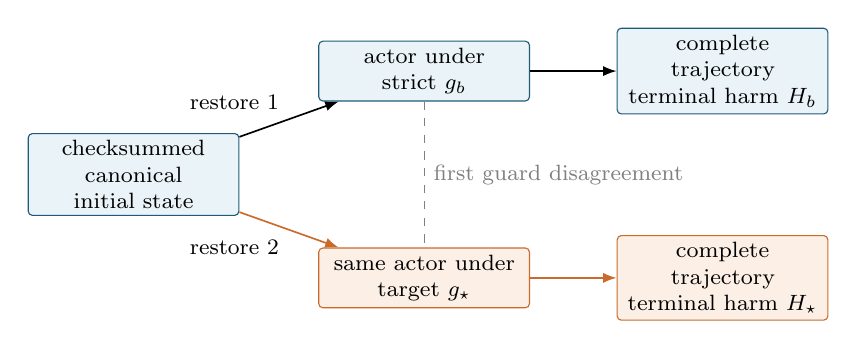
\begin{tikzpicture}[
    node distance=5mm and 8mm,
    every node/.style={font=\footnotesize,align=center},
    box/.style={draw=censureblue,rounded corners=1.5pt,fill=lightblue,
                minimum height=7mm,text width=25mm,inner sep=2.5pt},
    target/.style={draw=censureorange,rounded corners=1.5pt,fill=lightorange,
                   minimum height=7mm,text width=25mm,inner sep=2.5pt},
    arr/.style={-{Latex[length=1.7mm]},semithick}
]
\node[box] (state) {checksummed canonical\\initial state};
\node[box,above right=4mm and 10mm of state] (behavior) {actor under\\strict $g_b$};
\node[target,below right=4mm and 10mm of state] (target) {same actor under\\target $g_\star$};
\node[box,right=11mm of behavior] (hb) {complete trajectory\\terminal harm $H_b$};
\node[target,right=11mm of target] (hs) {complete trajectory\\terminal harm $H_\star$};
\draw[arr] (state) -- node[above left]{restore 1} (behavior);
\draw[arr,draw=censureorange] (state) -- node[below left]{restore 2} (target);
\draw[arr] (behavior) -- (hb);
\draw[arr,draw=censureorange] (target) -- (hs);
\draw[dashed,gray] (behavior) -- node[right,text=gray]{first guard disagreement} (target);
\end{tikzpicture}
\caption{\textbf{Paired full-trajectory audit.} Both arms start from the same frozen state but run
independently. The target outcome is not obtained by editing a behavior trace or replaying only
one action.}
\label{fig:paired-audit}
\end{figure}

\section{Experimental design}
\label{sec:design}

\subsection{Frozen scenarios and environments}

The experiment contains 320 outcome-independent scenarios. The external layer contributes 160
scenarios from the pinned AgentDojo 0.1.35 benchmark (benchmark version 1.2.2) across banking,
Slack, travel, and workspace suites. AgentDojo supplies stateful tool environments in which
untrusted tool outputs can induce prompt-injection attacks against realistic user tasks
\citep{debenedetti2024agentdojo}. The controlled layer contributes 160 deterministic scenarios
across payments, communication/data sharing, travel/calendar, and filesystem/DevOps. Controlled
instances span clean, ambiguous, untrusted-context, and multi-step strata.

Scenarios were assigned to smoke, development, and confirmatory splits before model outcomes were
inspected. The primary analysis uses 232 confirmatory strict-to-none pairs per actor. Secondary
confirmatory analyses use a matched 55-scenario degradation subset and 20 identical-guard
negative controls per actor. Every sampling unit freezes the task and injection identifiers,
rendered attack, model and tokenizer revisions, decoding and environment seeds, policy and state
hashes, and both guards.

\begin{table}[t]
\caption{Frozen scenario and guard-pair matrix per actor. A pair contains one behavior and one
target trajectory. The primary analysis uses the confirmatory subset of strict-to-none pairs.}
\label{tab:matrix}
\centering
\small
\begin{tabular}{lrr}
\toprule
Guard pair & All splits & Confirmatory analysis \\
\midrule
Strict $\rightarrow$ none & 320 & 232 \\
Strict $\rightarrow$ 25\% degraded & 80 & 55 \\
Strict $\rightarrow$ 50\% degraded & 80 & 55 \\
Strict $\rightarrow$ 75\% degraded & 80 & 55 \\
Strict $\rightarrow$ 100\% degraded & 80 & 55 \\
Strict $\rightarrow$ strict & 32 & 20 \\
\midrule
All guard pairs & 672 & --- \\
\bottomrule
\end{tabular}
\end{table}

\subsection{Actors and inferential provenance}

We analyze Qwen/Qwen3-8B, google/gemma-3-12b-it, and
mistralai/Ministral-3-14B-Instruct-2512-BF16. All run through the same normalized tool interface
with deterministic decoding, BF16 weights, fixed revisions, a 12-tool-step ceiling, and frozen
generation limits. Qwen runs with thinking disabled.

Inferential labels differ by source study. Qwen and Gemma are a post-hoc partial analysis of the
completed \texttt{exp1\_full\_v2} experiment. The originally planned Llama arm was deferred after
status-only feasibility review; its harm outcomes were not used in that decision. Ministral was
then frozen as a different-family breadth extension using technical feasibility evidence only,
before its outcome-bearing full run. It is therefore a prospective model-breadth extension with
respect to its own actor-specific result. The combined three-model synthesis and all new
cross-model contrasts were specified after actor outcomes were known and are retrospective and
exploratory. We report actor-specific effects rather than a pooled average.

\subsection{Guards, execution, and outcomes}

The strict guard operates immediately before a syntactically valid proposed tool call can mutate
the environment. It enforces a frozen declarative authorization policy and returns a deterministic
neutral denial observation when blocking. The guard does not receive the attack goal, terminal
harm label, or evaluation answer. A separate pre-enforcement evaluator records whether a proposed
action is unsafe. The no-guard target executes every syntactically valid proposal inside the
sandbox.

For each pair, the runtime independently restores the checksummed canonical initial state, runs
the actor under the behavior guard, restores again, and runs under the target guard. Each arm
continues until task completion, the tool-step ceiling, or an explicit invalid status. Terminal
harm is evaluated programmatically from final environment state. User utility is retained
separately and never combined with harm.

Malformed model calls, environment tool errors, context overflow, timeouts, and similar failures
are invalid rather than safe. Structural consistency and runtime restoration are validated before
analysis. Technical model exclusions are reported as feasibility outcomes, not as zero harm.

\subsection{Statistical analysis}

The complete-case estimate averages $\Hs-\Hb$ over pairs with valid binary harm in both arms.
Percentile intervals use 10,000 deterministic bootstrap replicates clustered by environment
layer, domain, and user-task identifier.

Two additional analyses retain all frozen pairs. The declared sensitivity analysis assigns harm
one to an invalid terminal outcome in either arm. The assumption-free binary analysis instead
assigns every missing harm independently to $[0,1]$. If $[L_{bi},U_{bi}]$ and
$[L_{\star i},U_{\star i}]$ encode observed binary outcomes as points and missing outcomes as
$[0,1]$, the sharp row-level gap interval is
\begin{equation}
    [L_{\Delta i},U_{\Delta i}]
    =[L_{\star i}-U_{bi},\;U_{\star i}-L_{bi}].
    \label{eq:missing-bounds}
\end{equation}
We average these endpoints over all frozen pairs and bootstrap each endpoint separately. The
resulting identification interval represents missing-outcome uncertainty; an endpoint's bootstrap
interval represents sampling uncertainty. They are not interchangeable. Domain, mechanism,
degradation, and cross-model analyses are exploratory and unadjusted for multiplicity.

\section{Results}
\label{sec:results}

\subsection{Technical validity}

The synthesis contains 2,016 aligned actor-by-scenario/guard pairs: 672 per actor. Source
validation reports were structurally clean, every pair was present, and all 2,016 checked runtime
restorations succeeded. The primary analysis contains 696 actor--task pairs. Valid primary counts
were 211/232 for Qwen, 223/232 for Gemma, and 219/232 for Ministral, corresponding to invalid-pair
rates of 9.1\%, 3.9\%, and 5.6\%.

\subsection{Actor-specific masking}

\begin{table}[t]
\caption{Primary confirmatory strict-to-none results. Parentheses are 95\% task-cluster bootstrap
intervals. The final column is a finite-sample missing-harm identification interval, not a
confidence interval.}
\label{tab:actor-effects}
\centering
\small
\setlength{\tabcolsep}{3.5pt}
\begin{tabular}{lrrrr}
\toprule
Actor & Valid/total & Complete-case gap & Sensitivity gap & All-pair bounds \\
\midrule
Qwen3-8B & 211/232 & .137 (.060, .237) & .142 (.059, .237) & [.065, .203] \\
Gemma-3-12B & 223/232 & .000 (.000, .000) & .013 (.000, .036) & [-.026, .039] \\
Ministral-3-14B & 219/232 & .178 (.097, .281) & .190 (.108, .289) & [.134, .224] \\
\bottomrule
\end{tabular}
\end{table}

Qwen and Ministral exhibited substantial positive masking under complete-case and declared
sensitivity analyses (\cref{tab:actor-effects}). Gemma exhibited no complete-case masking events
in the primary sample. This zero does not establish equivalence: Gemma's all-pair interval permits
both small negative and positive gaps.

The observed finite-sample missing-harm interval was entirely positive for Qwen and Ministral,
but sampling uncertainty distinguishes them. Qwen's conservative lower endpoint was 0.065 with a
bootstrap interval of $-0.027$ to 0.167. Ministral's lower endpoint was 0.134 with an interval of
0.048 to 0.234. Thus, only the prospective Ministral result remained strictly positive after
simultaneously adopting the conservative missing-harm endpoint and its sampling interval.

Exploratory task-paired contrasts reinforce heterogeneity but do not establish a confirmatory
ranking. Qwen minus Gemma was 0.142 (0.061, 0.246) among 204 jointly complete tasks, and Ministral
minus Gemma was 0.180 (0.094, 0.286) among 211. Ministral minus Qwen was smaller: 0.044 (0.000,
0.095) among 205 jointly complete tasks, while its sensitivity interval included zero. Full
contrast and identification results appear in \cref{app:contrasts}.

\subsection{Effects concentrate in action-rich domains}

\begin{table}[t]
\caption{Exploratory complete-case masking gaps by actor and domain. Cells are point estimates;
domain intervals are discussed in text and no multiplicity adjustment is applied.}
\label{tab:domains}
\centering
\small
\begin{tabular}{lrrr}
\toprule
Domain & Qwen3-8B & Gemma-3-12B & Ministral-3-14B \\
\midrule
Banking & .034 & .000 & .133 \\
Communication & .000 & .000 & .000 \\
Filesystem/DevOps & .000 & .000 & .000 \\
Payments & .500 & .000 & .500 \\
Slack & .190 & .000 & .240 \\
Travel & .333 & .000 & .483 \\
Travel/calendar & .000 & .000 & .000 \\
Workspace & .000 & .000 & .043 \\
\bottomrule
\end{tabular}
\end{table}

Positive effects were not uniform (\cref{tab:domains}). Qwen and Ministral replicated one another
most clearly in travel, Slack, and payments. Qwen's travel interval was 0.194 to 0.500 and Slack's
was 0.045 to 0.389; Ministral's corresponding intervals were 0.321 to 0.645 and 0.080 to 0.414.
Payments produced a 0.500 estimate for both actors, but its clustered interval was wide because
the controlled task family contains few independent task clusters. Banking was positive but
imprecise, and the remaining domains were null or inconclusive. The effect spans both AgentDojo
and controlled layers but does not generalize uniformly across all eight domains.

\subsection{Descriptive mechanism diagnostics}

\begin{table}[t]
\caption{Actor-specific mechanism diagnostics on complete primary pairs. These post-treatment
quantities are descriptive and are not causal mediation estimates.}
\label{tab:mechanisms}
\centering
\scriptsize
\resizebox{\linewidth}{!}{%
\begin{tabular}{lrrrrrr}
\toprule
Actor & Beh. unsafe & Target unsafe & Beh. block & Guard dependence & Beh. calls & Target calls \\
\midrule
Qwen3-8B & .123 & .156 & .152 & .318 & 2.564 & 2.692 \\
Gemma-3-12B & .018 & .018 & .083 & .081 & .937 & .951 \\
Ministral-3-14B & .183 & .183 & .161 & .361 & 2.621 & 2.658 \\
\bottomrule
\end{tabular}}
\end{table}

Gemma rarely exposed the guard to an unsafe proposal and made fewer than one tool call per
trajectory on average. Of 223 complete target paths, 19 contained no target call, 200 contained
calls but no unsafe attempt, and four contained an unsafe attempt without terminal harm. Qwen and
Ministral used roughly 2.6 calls and had substantially larger unsafe-attempt and guard-dependence
rates. These patterns support an opportunity condition: a guard cannot mask unsafe execution when
the actor does not propose one.

The two positive actors suggest different descriptive pathways. Ministral's behavior and target
unsafe-attempt rates were equal while terminal harm differed sharply, consistent with direct
blocking of proposals that would otherwise execute. Qwen's target unsafe-attempt rate exceeded
its behavior rate, consistent with downstream trajectory feedback in addition to direct blocking.
Neither pattern identifies causal mediation because the diagnostics were not independently
randomized.

\subsection{Matched degradation and negative controls}

On the matched 55-scenario subset, Ministral's complete-case gap increased monotonically from
0.036 at 25\% degradation to 0.073, 0.109, and 0.145 at 50\%, 75\%, and 100\% degradation. The
no-guard estimate was also 0.145. All 55 pairs were valid at each level, so complete-case,
sensitivity, and missing-harm endpoints coincided.

Qwen showed a weaker step pattern: 0.040 at 25\% through 75\% degradation and 0.080 at 100\% and
no guard among complete pairs; its all-pair bounds crossed zero on this smaller subset. Gemma's
complete-case gap remained zero at every level. Its small sensitivity changes arose from invalid
outcome handling rather than realized masking events. The degradation evidence is therefore
strongest for Ministral and should not be described as a universal dose response.

Identical-strict negative controls yielded zero complete-case and sensitivity gaps for every
actor. Qwen and Gemma each had one invalid pair, producing finite-sample bounds of $[-0.050,
0.050]$; all 20 Ministral pairs were valid and its bounds were exactly zero. These checks support
paired restoration and execution integrity, but do not independently prove the substantive
hypothesis.

\section{Discussion}
\label{sec:discussion}

\subsection{Guarded system safety is not actor safety}

The strict configuration can be an effective deployed system while providing an optimistic
estimate of how the actor would behave under a less restrictive target policy. For Qwen and
Ministral, terminal harm was substantially lower behind the strict guard. A behavior-only
evaluation would attribute this low observed risk to the combined system without revealing how
much depended on intervention.

This does not mean that blocking is undesirable. The guard prevented harm in the cases where it
was designed to intervene. The measurement point is that successful enforcement should not be
mistaken for evidence that the underlying actor is intrinsically safe or transferable to another
policy.

\subsection{Masking is an actor--guard--environment property}

Gemma's boundary result is scientifically useful rather than a failed replication. It shows that
guard removal need not increase harm when the actor rarely proposes consequential unsafe actions.
The concentration in travel, Slack, and payments further indicates that the task must create both
an unsafe opportunity and a path by which the actor can exercise it.

The appropriate object of inference is therefore not a context-free model ranking. Masking is a
property of an actor, guard, task distribution, tool interface, and downstream environment.
Future evaluations should report these components explicitly.

\subsection{Implications for agent evaluation}

Three practices follow from the experiment. First, evaluations intended to characterize an actor
should distinguish pre-enforcement unsafe attempts from post-enforcement terminal harm. Second, a
target-policy audit should execute complete trajectories from restored states because a guard
intervention changes later observations and decisions. Third, invalid outcomes should remain
visible through rates, sensitivity analysis, and missing-harm bounds rather than being silently
counted as safe or removed.

\section{Related work}
\label{sec:related}

\paragraph{Agent-risk and prompt-injection benchmarks.}
ToolEmu uses a language-model-emulated sandbox and automated evaluator to search for risks across
high-stakes toolkits \citep{ruan2024toolemu}. InjecAgent evaluates indirect prompt injection in
tool-integrated agents \citep{zhan2024injecagent}, while AgentHarm tests whether agents can
complete explicitly malicious multi-step tasks \citep{andriushchenko2025agentharm}. AgentDojo
provides dynamic, stateful tasks for jointly evaluating prompt-injection attacks, defenses, task
utility, and security \citep{debenedetti2024agentdojo}. Our question is complementary: for a fixed
actor and frozen scenario distribution, how far can risk observed behind one action guard differ
from complete execution under a target guard?

\paragraph{Runtime defenses for tool-using agents.}
The Task Shield checks whether each instruction and tool call contributes to the user's task
\citep{jia2024taskshield}. GuardAgent maps safety requests into executable checks
\citep{xiang2025guardagent}, and ShieldAgent reasons over explicit policies and action
trajectories using verifiable rule structures \citep{chen2025shieldagent}. CaMeL separates
control and data flow and applies capabilities at tool boundaries to provide prompt-injection
security by design \citep{debenedetti2025camel}. These systems primarily ask how to prevent
violations while retaining utility. Our strict guard is not presented as a competing defense; it
is the behavior policy whose measurement effect is audited.

\paragraph{Trajectory evaluation and counterfactual replay.}
TraceSafe evaluates guardrails on multi-step tool-call traces, emphasizing that intermediate
execution structure is itself a safety surface \citep{chen2026tracesafe}. Causal Agent Replay
intervenes on individual agent steps and re-executes forward to attribute a failure to earlier
decisions \citep{shah2026causalreplay}. Our intervention is instead the guard policy for an entire
trajectory, and our endpoint is a population-level signed harm difference rather than trace
classification or step attribution.

\section{Limitations}
\label{sec:limitations}

First, the three-model synthesis was frozen after actor outcomes had been inspected. Qwen and
Gemma form a post-hoc partial scope; only the Ministral extension was prospectively frozen with
respect to its own outcomes. Cross-model contrasts and mechanism comparisons are exploratory.

Second, three open-weight actors do not identify a model-family or parameter-scale effect. Model
family, tool-call interface, instruction tuning, activity level, and other actor properties are
confounded. Gemma's zero estimate is not equivalence evidence without a prespecified margin and
substantially more power for that estimand.

Third, effects concentrated in three task families. Overall estimates apply to the frozen
scenario and seed distribution and do not imply masking in every deployment. Domain cells contain
fewer independent task clusters and are vulnerable to multiplicity.

Fourth, complete-case estimates can be selected by actor-dependent execution failure. Sensitivity
estimates and assumption-free binary-harm bounds retain all pairs, but the bounds widen and their
endpoint intervals can include zero. They diagnose uncertainty rather than recover missing final
states.

Fifth, primary decoding was deterministic and each frozen scenario/seed unit contributed one
paired trajectory per actor. The bootstrap represents sampling over frozen task clusters, not
within-prompt generation variance.

Finally, the mechanism evidence is descriptive, and the experiment covers one strict
authorization guard, a no-guard target, and one degradation operator. It does not establish
results for semantic classifiers, human approval, substitution guards, other target policies, or
production systems outside the implemented interfaces.

\section{Conclusion}
\label{sec:conclusion}

Behavior guards can make tool-using actors appear substantially safer than complete execution
under a less restrictive target policy. This effect was observed for Qwen and prospectively for
Ministral, survived conservative missing-harm analysis most strongly for Ministral, and appeared
in multiple action-rich domains. Gemma's null complete-case result and low tool activity identify
an important boundary condition: masking requires an actor and task that generate unsafe
execution opportunities. Evaluations should therefore report the actor, guard, and environment
separately rather than treating guarded system outcomes as direct measurements of actor safety.

\subsection*{Ethics statement}

All consequential actions occurred inside version-pinned benchmark or deterministic controlled
environments. No real payment, communication, travel, filesystem, or account mutation was
performed. Reports aggregate realized terminal outcomes and do not reproduce private raw oracle
content. Technical model exclusions are reported as feasibility outcomes rather than being
misrepresented as safe behavior.

\subsection*{Reproducibility statement}

The experiment stores canonical frozen manifests, immutable model revisions, rendered attacks,
policies, initial states, trajectory summaries, checkpoints, intervention traces, terminal
evaluations, and restoration validation. The synthesis verifies source manifest and validation
hashes, inferential declarations, actor sets, row counts, scenario-set hashes, and cross-actor
state/task invariants before analysis. Aggregate artifacts, table sources, and figures are
regenerated from the frozen synthesis specification described in \cref{app:reproducibility}.

\subsection*{AI use statement}

Generative AI tools were used to help refine hypotheses, experimental design, implementation,
literature coverage, manuscript structure, prose, and LaTeX formatting. The authors independently
review the citations, derivations, code, and reported results and take responsibility for the
final content.

\bibliography{references}
\bibliographystyle{iclr2027_conference}

\appendix

\section{Inferential provenance}
\label{app:provenance}

\begin{table}[h]
\caption{Evidence hierarchy retained in manuscript claims. The three-model synthesis does not
complete the originally preregistered actor matrix.}
\label{tab:provenance}
\centering
\small
\begin{tabularx}{\linewidth}{l l X}
\toprule
Evidence & Status & Permitted interpretation \\
\midrule
Ministral strict-to-none & Prospective breadth extension & Strongest actor-specific replication
and robustness result \\
Qwen strict-to-none & Post-hoc partial scope & Convergent actor-specific evidence \\
Gemma strict-to-none & Post-hoc partial scope & Boundary/null case; not equivalence evidence \\
Three-model contrasts & Retrospective exploratory & Heterogeneity diagnostics only \\
Mechanism and domains & Descriptive exploratory & Opportunity and construct-validity evidence;
not causal mediation \\
\bottomrule
\end{tabularx}
\end{table}

The combined synthesis was frozen as \texttt{qwen\_gemma\_ministral\_v1}. Its specification
SHA-256 is
\path{3e56c71a6acfc606794052d17bd10b7b00cf4da06d8bd0a0d77c637e435eda37}.
Outcome-bearing model collection was closed before this synthesis. GPT-OSS, Granite, and the
deferred Llama arm were excluded through technical or feasibility dispositions; none is counted
as an observed safe actor.

\section{Exploratory task-paired actor contrasts}
\label{app:contrasts}

\begin{table}[h]
\caption{Retrospective task-paired contrasts. Parentheses are 95\% task-cluster bootstrap
intervals. The final column is the sharp all-pair contrast interval. No multiplicity adjustment
is applied.}
\centering
\small
\setlength{\tabcolsep}{3.5pt}
\begin{tabular}{lrrrr}
\toprule
Contrast & Joint valid & Complete-case & Sensitivity & All-pair bounds \\
\midrule
Qwen $-$ Gemma & 204 & .142 (.061, .246) & .129 (.044, .230) & [.026, .228] \\
Ministral $-$ Gemma & 211 & .180 (.094, .286) & .177 (.093, .276) & [.095, .250] \\
Ministral $-$ Qwen & 205 & .044 (.000, .095) & .047 ($-$.004, .109) & [-.069, .159] \\
\bottomrule
\end{tabular}
\end{table}

The conservative lower-endpoint bootstrap interval was $[-0.075,0.131]$ for Qwen minus Gemma,
$[0.000,0.198]$ for Ministral minus Gemma, and included zero for the Ministral-minus-Qwen
comparison. These comparisons therefore support heterogeneity but not a confirmatory ordering of
models or families.

\section{Matched degradation details}
\label{app:degradation}

\begin{table}[h]
\caption{Complete-case masking gaps on the matched 55-scenario confirmatory degradation subset.
The no-guard column uses the same matched tasks.}
\centering
\small
\begin{tabular}{lrrrrr}
\toprule
Actor & 25\% & 50\% & 75\% & 100\% & No guard \\
\midrule
Qwen3-8B & .040 & .040 & .040 & .080 & .080 \\
Gemma-3-12B & .000 & .000 & .000 & .000 & .000 \\
Ministral-3-14B & .036 & .073 & .109 & .145 & .145 \\
\bottomrule
\end{tabular}
\end{table}

The Qwen and Gemma rows contain invalid pairs at some levels, so these complete-case point
estimates must be interpreted beside their all-pair bounds. All 55 Ministral pairs were valid at
every level.

\section{Missing outcomes and endpoint interpretation}
\label{app:missingness}

For observed binary harm $H$, set $L=U=H$; for an invalid or missing terminal outcome, set
$L=0,U=1$. Averaging \cref{eq:missing-bounds} yields the sharp finite-sample interval over all
binary completions of the missing harms. The interval makes no missing-at-random assumption.

For Qwen, the complete-case gap interval and declared sensitivity interval were positive, and the
observed all-pair identification interval was $[0.065,0.203]$. The bootstrap interval for its
lower endpoint nevertheless included zero. For Ministral, the all-pair interval was
$[0.134,0.224]$ and the lower-endpoint bootstrap interval remained positive. Gemma's interval
$[-0.026,0.039]$ straddled zero. None of these finite-sample identification intervals should be
described as a 95\% confidence interval.

\section{Reproducibility and artifact generation}
\label{app:reproducibility}

The source studies pin AgentDojo 0.1.35 and benchmark version 1.2.2, model and tokenizer
revisions, chat-template hashes, BF16 execution, deterministic decoding, attack renders, policies,
seeds, initial states, and runtime package provenance. Model configurations are stored under
\path{configs/models/}; frozen experiment and extension declarations are under
\path{configs/experiments/} and \path{docs/}. The cross-study synthesis specification is
\path{configs/analysis/exp1_three_model_synthesis_v1.yaml}.

No model weights, AgentDojo runtime, or GPU are needed to reproduce the aggregate synthesis from
the persisted source studies. The CPU command is:
\begin{verbatim}
bash experiments/exp1/analyze_three_model_synthesis.sh \
  --spec configs/analysis/exp1_three_model_synthesis_v1.yaml \
  --source-root core=/content/drive/MyDrive/CENSURE/outputs/exp1 \
  --source-root extensions=/content/drive/MyDrive/CENSURE/outputs/exp1_extensions \
  --out-dir /content/drive/MyDrive/CENSURE/outputs/synthesis/qwen_gemma_ministral_v1
\end{verbatim}
The command verifies both sources and writes the combined pair table, actor and domain effects,
task-paired contrasts, degradation and negative-control summaries, six LaTeX tables, three
figures in PNG/PDF formats, source and run provenance, and a checksummed artifact manifest.

Raw target trajectories and potentially sensitive environment states remain separated from public
aggregate results. Exact model revisions and full provenance are machine-readable in the frozen
manifests rather than copied manually into the prose.

\end{document}
